%!TEX TS-program = xelatex
\documentclass[12pt, a4paper, oneside]{article}

\usepackage{amsmath,amsfonts,amssymb,amsthm,mathtools}  % пакеты для математики

\usepackage[utf8]{inputenc} % задание utf8 кодировки исходного tex файла
\usepackage[british,russian]{babel} % выбор языка для документа

\usepackage{fontspec}         % пакет для подгрузки шрифтов
\setmainfont{Helvetica}   % задаёт основной шрифт документа

% why do we need \newfontfamily:
% http://tex.stackexchange.com/questions/91507/
\newfontfamily{\cyrillicfonttt}{Helvetica}
\newfontfamily{\cyrillicfont}{Helvetica}
\newfontfamily{\cyrillicfontsf}{Helvetica}

\usepackage{unicode-math}     % пакет для установки математического шрифта
\setmathfont{Neo Euler}      % шрифт для математики
% \setmathfont[math-style=ISO]{Asana Math}
% Можно делать смену начертания с помощью разных стилей

% Конкретный символ из конкретного шрифта
% \setmathfont[range=\int]{Neo Euler}

%%%%%%%%%% Работа с картинками %%%%%%%%%
\usepackage{graphicx}                  % Для вставки рисунков
\usepackage{graphics}
\graphicspath{{images/}{pictures/}}    % можно указать папки с картинками
\usepackage{wrapfig}                   % Обтекание рисунков и таблиц текстом

%%%%%%%%%%%%%%%%%%%%%%%% Графики и рисование %%%%%%%%%%%%%%%%%%%%%%%%%%%%%%%%%
\usepackage{tikz, pgfplots}  % язык для рисования графики из latex'a

%%%%%%%%%% Гиперссылки %%%%%%%%%%
\usepackage{xcolor}              % разные цвета

\usepackage{hyperref}
\hypersetup{
	unicode=true,           % позволяет использовать юникодные символы
	colorlinks=true,       	% true - цветные ссылки, false - ссылки в рамках
	urlcolor=blue,          % цвет ссылки на url
	linkcolor=red,          % внутренние ссылки
	citecolor=green,        % на библиографию
	pdfnewwindow=true,      % при щелчке в pdf на ссылку откроется новый pdf
	breaklinks              % если ссылка не умещается в одну строку, разбивать ли ее на две части?
}


\usepackage{todonotes} % для вставки в документ заметок о том, что осталось сделать
% \todo{Здесь надо коэффициенты исправить}
% \missingfigure{Здесь будет Последний день Помпеи}
% \listoftodos --- печатает все поставленные \todo'шки

\usepackage{enumitem} % дополнительные плюшки для списков
%  например \begin{enumerate}[resume] позволяет продолжить нумерацию в новом списке

\usepackage[paper=a4paper, top=20mm, bottom=15mm,left=20mm,right=15mm]{geometry}
\usepackage{indentfirst}       % установка отступа в первом абзаце главы

\usepackage{setspace}
\setstretch{1.15}  % Межстрочный интервал
\setlength{\parskip}{4mm}   % Расстояние между абзацами
% Разные длины в латехе https://en.wikibooks.org/wiki/LaTeX/Lengths


\usepackage{xcolor} % Enabling mixing colors and color's call by 'svgnames'

\definecolor{MyColor1}{rgb}{0.2,0.4,0.6} %mix personal color
\newcommand{\textb}{\color{Black} \usefont{OT1}{lmss}{m}{n}}
\newcommand{\blue}{\color{MyColor1} \usefont{OT1}{lmss}{m}{n}}
\newcommand{\blueb}{\color{MyColor1} \usefont{OT1}{lmss}{b}{n}}
\newcommand{\red}{\color{LightCoral} \usefont{OT1}{lmss}{m}{n}}
\newcommand{\green}{\color{Turquoise} \usefont{OT1}{lmss}{m}{n}}

\usepackage{titlesec}
\usepackage{sectsty}
%%%%%%%%%%%%%%%%%%%%%%%%
%set section/subsections HEADINGS font and color
\sectionfont{\color{MyColor1}}  % sets colour of sections
\subsectionfont{\color{MyColor1}}  % sets colour of sections

%set section enumerator to arabic number (see footnotes markings alternatives)
\renewcommand\thesection{\arabic{section}.} %define sections numbering
\renewcommand\thesubsection{\thesection\arabic{subsection}} %subsec.num.

%define new section style
\newcommand{\mysection}{
	\titleformat{\section} [runin] {\usefont{OT1}{lmss}{b}{n}\color{MyColor1}} 
	{\thesection} {3pt} {} } 


%	CAPTIONS
\usepackage{caption}
\usepackage{subcaption}
%%%%%%%%%%%%%%%%%%%%%%%%
\captionsetup[figure]{labelfont={color=Turquoise}}

\usepackage[normalem]{ulem}  % для зачекивания текста

\pagestyle{empty}

\begin{document}

\section*{Задание 8 (Эпилог)  }

\subsection*{[10]   Упражнение 1 (Пожалуй, самый сложный пакет в вашей жизни ) }

	Суть этого упражнения сводится к тому, что вы должны заставить работать пакет minted.  Этот пакет вы в будущем будете использовать для оформления кода.  Напоминаю, что этот пакет написан на Python. Это означает, что для использования minted должен быть установлен Python. \textbf{Следуя инструкции ниже, установите minted.} 

\textbf{Windows:}

\begin{enumerate}
	\item Устанавливаем на компьютер Python. Лучше всего поставить дистрибутив, который называется \href{https://docs.continuum.io/anaconda/install}{Anaconda.} Этот дистрибутив включает в себя все основные пакеты, которые необходимы для работы с питоном. 
	
	\item Открываем консоль. Для этого жмём \texttt{win+R}, вводим в открывшемся окне \texttt{cmd}, жмём \texttt{enter}.  Открывается командная строка. 
	
	\item Прописываем в командной строке \texttt{pip install Pygments}
	
	\item Команда выше установила на наш компьютер питоновский пакет, который будет раскрашивать код в \LaTeX{}. Теперь нужно настроить texstudio. Заходим в настройки и там прописываем в графе  XeLatex: \newline  \texttt{Xelatex -shell-escape -synctex=1 -interaction=nonstopmode \%.tex`}
	
	\item Эта команда подключает к теху внешние пакеты. В нашем случае это Pygments. 
\end{enumerate} 


\textbf{Linux (Ubuntu 16):}

\begin{enumerate}
	\item Если честно, то в Anaconda много бесполезного хлама. И лучше приручать змей вручную. Но не на Windows. Жмём \texttt{ctrl+alt+T}, открывается терминал. 
	\item Убеждаемся, что установлен Python, вбивая в терминале \texttt{python --version}, а он установлен, потому что половина системы на нём написана.
	\item Убеждаемся, что установлен pip, вбивая  \texttt{pip --version}. Если он не установлен, то ставим его!  \texttt{sudo apt-get install python-pip}.
	\item Устанавливаем наш пакет  \texttt{sudo pip install Pygments}
	\item Заходим в настройки texmaker и там прописываем в графе  XeLatex:  \newline \texttt{Xelatex -shell-escape -synctex=1 -interaction=nonstopmode \%.tex`}
\end{enumerate} 

\textbf{Mac:}

\begin{enumerate}
	\item Оказывается, у вас на macOS уже стоит python. Еси открыть терминал, то можно убедиться в этом, прописав \texttt{python --version}
	\item Убеждаемся, что установлен pip, вбивая  \texttt{pip --version}. Если он не установлен, то ставим его!  
	\item Устанавливаем наш пакет  \texttt{sudo pip install Pygments}
	\item  Готово! Теперь, если вы спросите \texttt{which pygmentize}, то  ответ должен быть такой  \texttt{pygmentize is /usr/local/bin/pygmentize}
	\item Теперь можно запускать техмейкер/техстудио/техпад, подключать minted и, если вы не забыли в настройках  в графе  XeLatex:  подписать  \texttt{Xelatex -shell-escape -synctex=1 -interaction=nonstopmode \%.tex`}, то всё должно работать.
\end{enumerate} 


После всех этих действий вы должны почувствовать себя супермега программистом. Дело осталось за малым. Создаём теховский документ, подключаем пакет minted и используем окружение minted. Вы ещё не забыли, что задание состояло в том, что нужно оформить какой-нибудь кусочек своего кода с помощью minted? Именно за оформление любого кода вы и получите свои честно заработанные баллы. 


\subsection*{[респект ]  Упражнение 2  (Наклеечи)}

Каждые полгода в Москве проходит \href{http://datafest.ru/}{Датафест.} Одно из самых крупных собраний датамайнеров. На каждый датафест печатается партия отличных наклеек! Главная особенность этих наклеек состоит в том, что их хотят все.

\begin{center}
	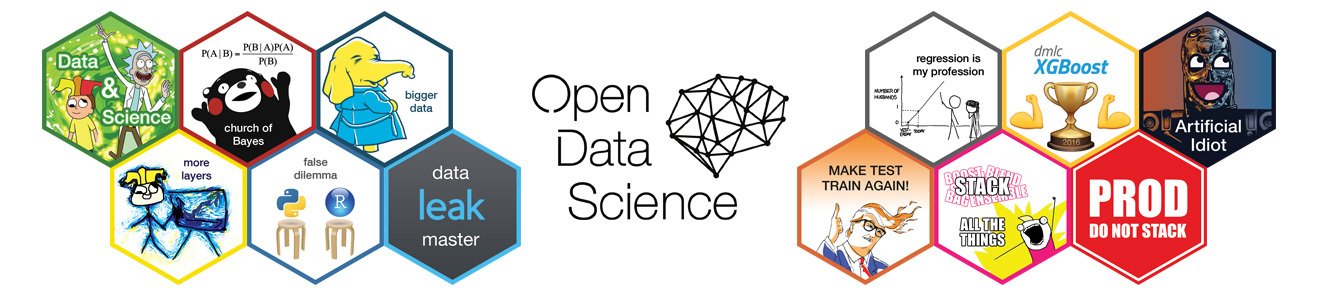
\includegraphics[scale=0.35]{DF.jpg}
\end{center}

\todo[inline]{Переписать на актуальную инфу}

Новый датафест пройдёт 28 апреля. Если интересуетесь эконометрикой и ML, непременно посетите его... 

В мае будет проходить ещё одна прикольная штука в рамках факультета: работающие для безработных. К прошлой такой штуке мы печатали партию наклеек, нарисованных на курсе по теху. В этот раз я такое задание не давал, так как оно жрет ещё больше времени, чем остальные задания. Тем не менее, если вы хотите, чтобы ваша наклейка пополнила ряды стикеров на ноутах, вы можете попробовать нарисовать её в TikZ, если вы извращенец или в фотошопе, если вы не извращенец. 

Идеология наклеек следующая: на наклейке должен быть либо общеизвестный символ, либо тонкая профессиональная шутка. Например, если вы рисуете макроэкономическую наклеечку, то любой другой случайно заметивший её макроэкономист, например работающий в ЦБ, должен понять нарисованную шутку и захотеть такую наклейку себе. Более того, вы сами должны хотеть прилепить такую наклейку на крышку своего ноута или на другое видное место.



\subsection*{[Бесконечно ценно] Упражнение n+1 }

\textbf{[Счётная ценность]}  Установите Atom, настройте его. Научитесь собирать в нём файлы. Поэкспериментируйте с разными пакетами. Попробуйте Rshiny. Влюбитесь в него.  

\textbf{[Ценность мощности континуум]}  Создайте на Git свой собственный репозиторий. Скачейте какой-нибудь удобный графический редактор для него. Поэкспериментируйте с созданием своей странички или даже своего блога. Творите добро и выкладывайте его в свободный доступ!

\textbf{[Ценность мощности более чем континуум]} Удалите Windows. Навсегда удалите. Даже если у вас сейчас Mac или Linux, ворвитесь в Mвидео, найдите компьютер с Windows и удалите его. Установите любой дистрибутив Linux. (Можно купить Mac. Можно даже купить его для меня.) Посмотрите вводный курс о Linux, например на stepic.org. Получайте удовольствие от изучения своего компа. Ну хотябы параллельно поставьте. Или на старый комп. Пробуйте, чёрт возьми что-то новое! И не забывайте развиваться, чтобы было куда деградировать! :) 

\end{document} 
